\section{实验结果与分析}

\subsection{k-means聚类效果}

分别生成$2$簇、$3$簇、$4$簇数据,数据的真实情况与通过k-means聚类情况如图。其中深蓝色点代表每一个聚类的中心点。由于颜色是按照k-means迭代中心点$\mu$的位置生成的,因此有可能两侧颜色不匹配,这属于正常现象。
\begin{figure}[htbp]
    \begin{minipage}[t]{0.5\linewidth}
        \centering
        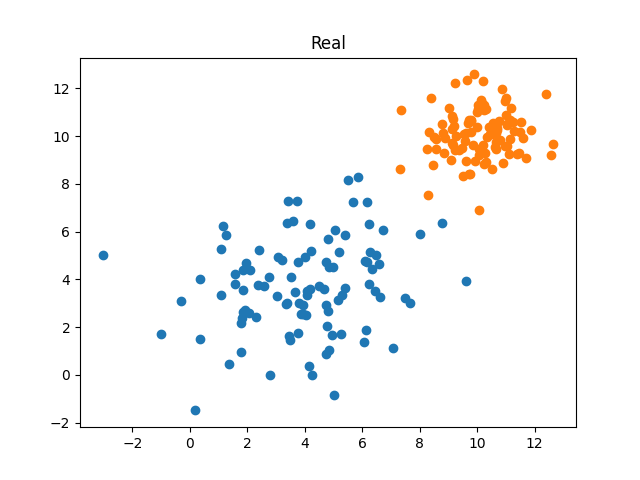
\includegraphics[width=\textwidth]{figures/Figure_1.png}
        \caption{$2$簇数据时的真实情况}
    \end{minipage}
    \begin{minipage}[t]{0.5\linewidth}
        \centering
        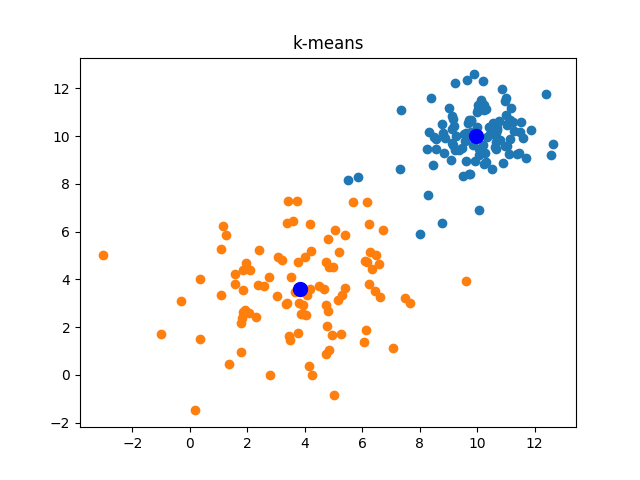
\includegraphics[width=\textwidth]{figures/Figure_2.png}
        \caption{$2$簇数据时用k-means的聚类情况}
    \end{minipage}
\end{figure}
\begin{figure}[htbp]
    \begin{minipage}[t]{0.5\linewidth}
        \centering
        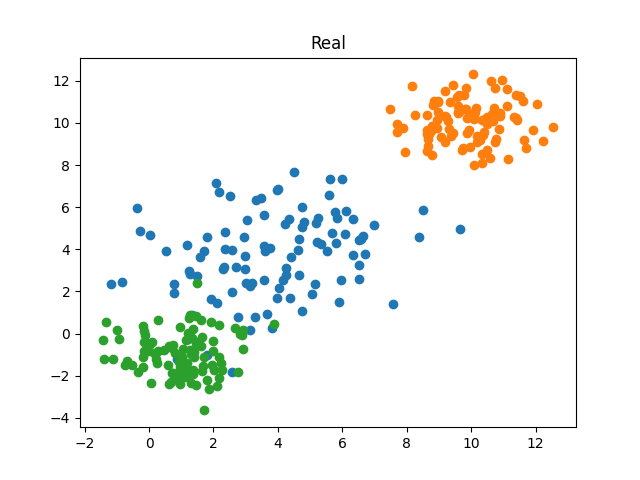
\includegraphics[width=\textwidth]{figures/Figure_3.png}
        \caption{$3$簇数据时的真实情况}
    \end{minipage}
    \begin{minipage}[t]{0.5\linewidth}
        \centering
        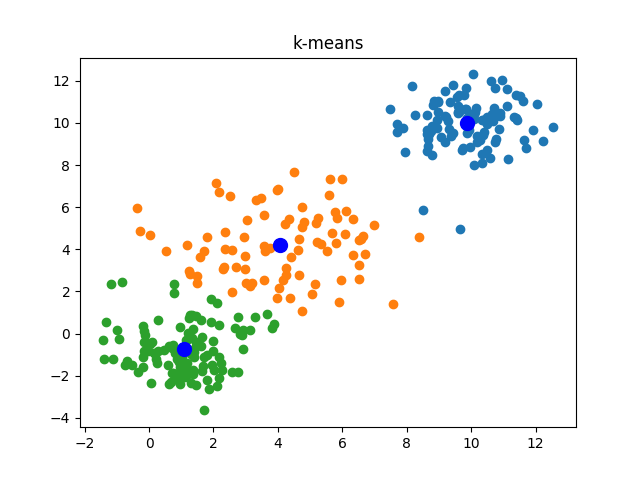
\includegraphics[width=\textwidth]{figures/Figure_4.png}
        \caption{$3$簇数据时用k-means的聚类情况}
    \end{minipage}
\end{figure}
\begin{figure}[htbp]
    \begin{minipage}[t]{0.5\linewidth}
        \centering
        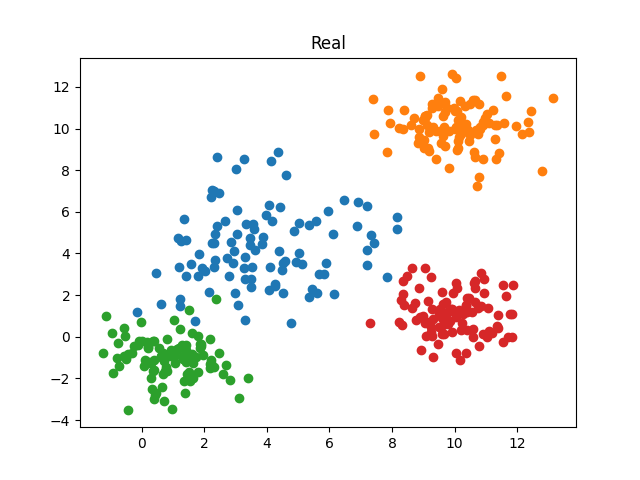
\includegraphics[width=\textwidth]{figures/Figure_5.png}
        \caption{$4$簇数据时的真实情况}
    \end{minipage}
    \begin{minipage}[t]{0.5\linewidth}
        \centering
        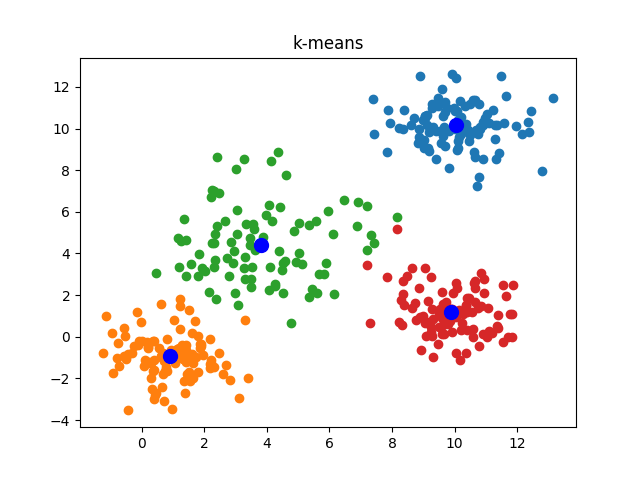
\includegraphics[width=\textwidth]{figures/Figure_6.png}
        \caption{$4$簇数据时用k-means的聚类情况}
    \end{minipage}
\end{figure}
从以上6张图可见k-means聚类效果较好。

\subsection{GMM-EM聚类效果}

生成$2$簇数据,数据的真实情况、通过k-means聚类情况、通过GMM-EM聚类情况如图。

\begin{figure}[htbp]
    \begin{minipage}[t]{0.3\linewidth}
        \centering
        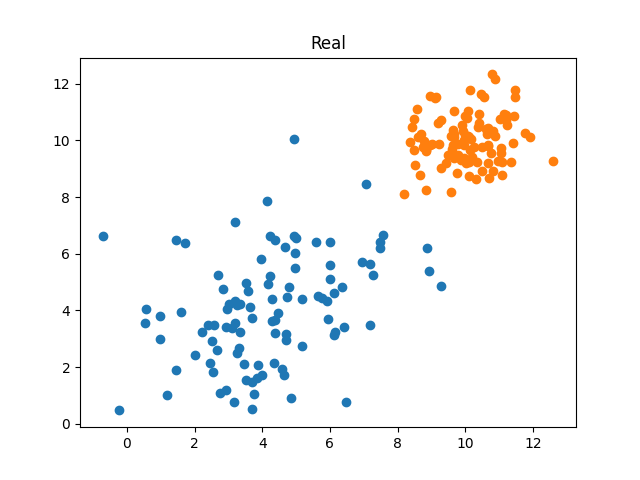
\includegraphics[width=\textwidth]{figures/Figure_7.png}
        \caption{$2$簇数据时的真实情况}
    \end{minipage}
    \begin{minipage}[t]{0.3\linewidth}
        \centering
        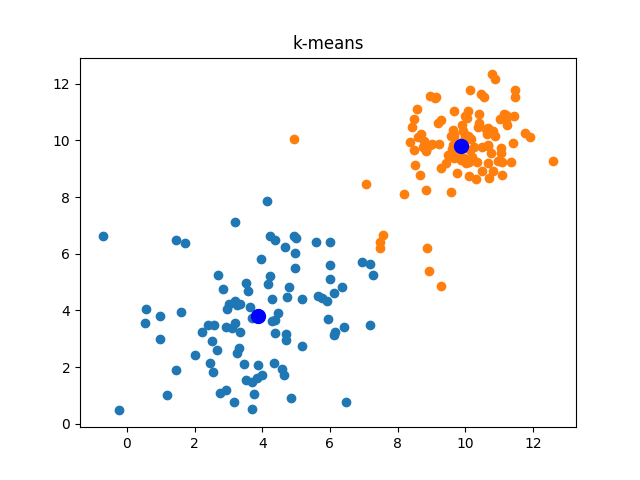
\includegraphics[width=\textwidth]{figures/Figure_8.png}
        \caption{$2$簇数据时用k-means的聚类情况}
    \end{minipage}
    \begin{minipage}[t]{0.3\linewidth}
        \centering
        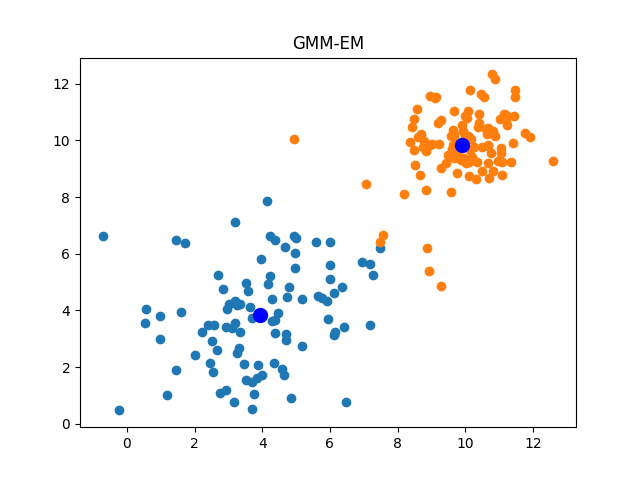
\includegraphics[width=\textwidth]{figures/Figure_9.png}
        \caption{$2$簇数据时用GMM-EM的聚类情况}
    \end{minipage}
\end{figure}

此时对训练的GMM-EM模型进行测试,测试数据集使用500个点,结果如图\ref{cluster2-test}。

\begin{figure}[htbp]
    \centering
    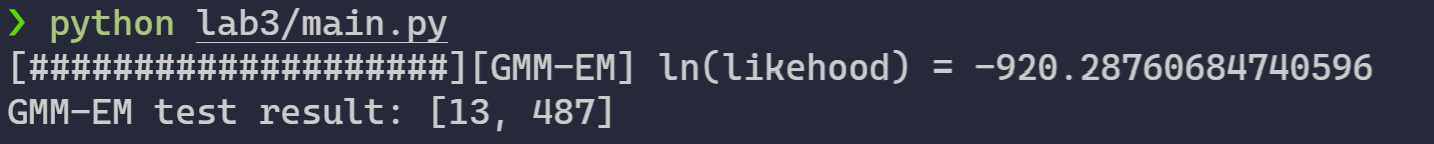
\includegraphics[width=0.7\textwidth]{figures/Figure_10.png}
    \caption{$2$簇数据时用GMM-EM的测试结果}
    \label{cluster2-test}
\end{figure}

图\ref{cluster2-test}其表示这500个1号类的点,有13个被分到0号簇,有487个被分到1号簇,准确率为$97.4\%$。

生成$4$簇数据,数据的真实情况、通过k-means聚类情况、通过GMM-EM聚类情况如图。

\begin{figure}[htbp]
    \begin{minipage}[t]{0.3\linewidth}
        \centering
        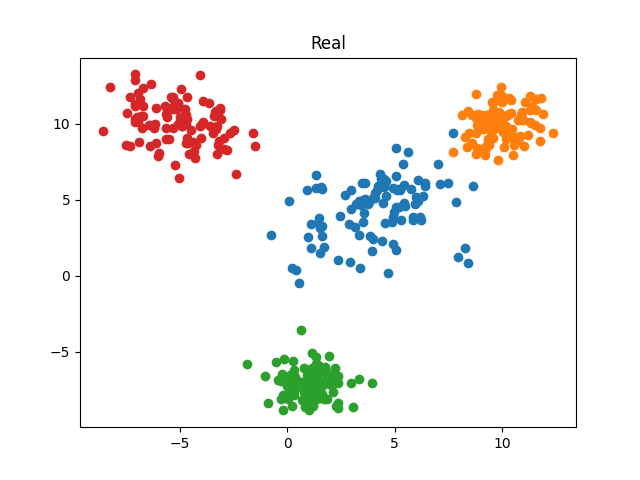
\includegraphics[width=\textwidth]{figures/Figure_11.png}
        \caption{$4$簇数据时的真实情况}
    \end{minipage}
    \begin{minipage}[t]{0.3\linewidth}
        \centering
        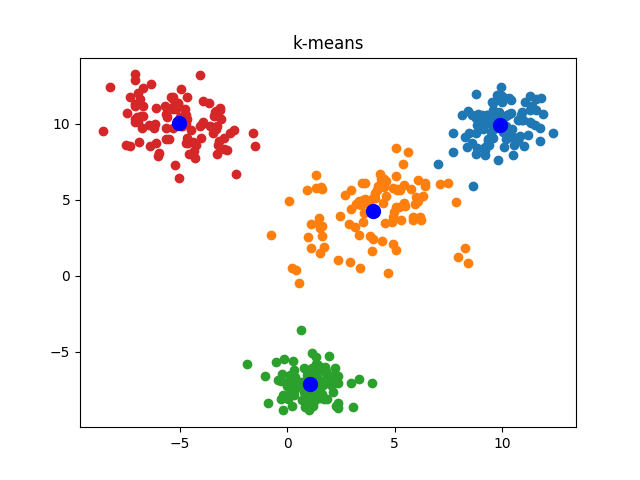
\includegraphics[width=\textwidth]{figures/Figure_12.png}
        \caption{$4$簇数据时用k-means的聚类情况}
    \end{minipage}
    \begin{minipage}[t]{0.3\linewidth}
        \centering
        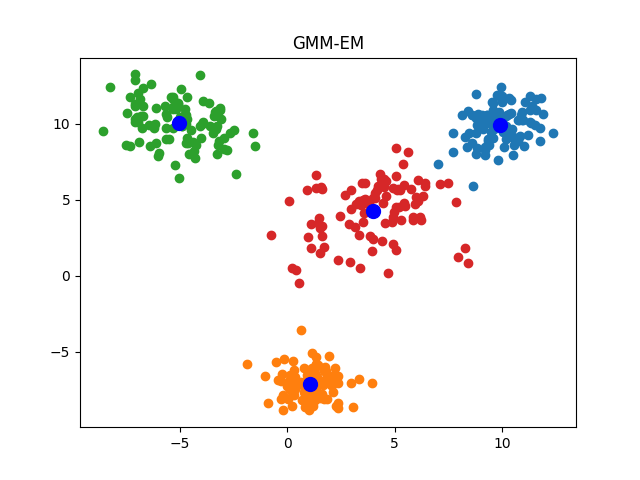
\includegraphics[width=\textwidth]{figures/Figure_13.png}
        \caption{$4$簇数据时用GMM-EM的聚类情况}
    \end{minipage}
\end{figure}

此时对训练的GMM-EM模型进行测试,测试数据集使用500个点,结果如图\ref{cluster4-test}。

\begin{figure}[htbp]
    \centering
    
\includegraphics[width=0.7\textwidth]{figures/Figure_14.png}
    \caption{$4$簇数据时用GMM-EM的测试结果}
    \label{cluster4-test}
\end{figure}

图\ref{cluster4-test}表示这500个3号类的点,有15个被分到0号簇,有2个被分到1号簇,有483个被分到3号簇,准确率为$96.6\%$,略高于k-means。这是由于k-means假设数据呈球状分布,而GMM使用多元高斯分布做更加普遍的假设。当样本各个维度间的相关系数不为0时,k-means的假设不成立,所以聚类的准确率有所下降。

下边对执行GMM-EM算法过程中对数似然函数进行分析。生成4簇数据,使用GMM-EM进行聚类,每次迭代的对数似然如图。

\begin{figure}[htbp]
    \begin{minipage}[t]{0.5\linewidth}
        \centering
        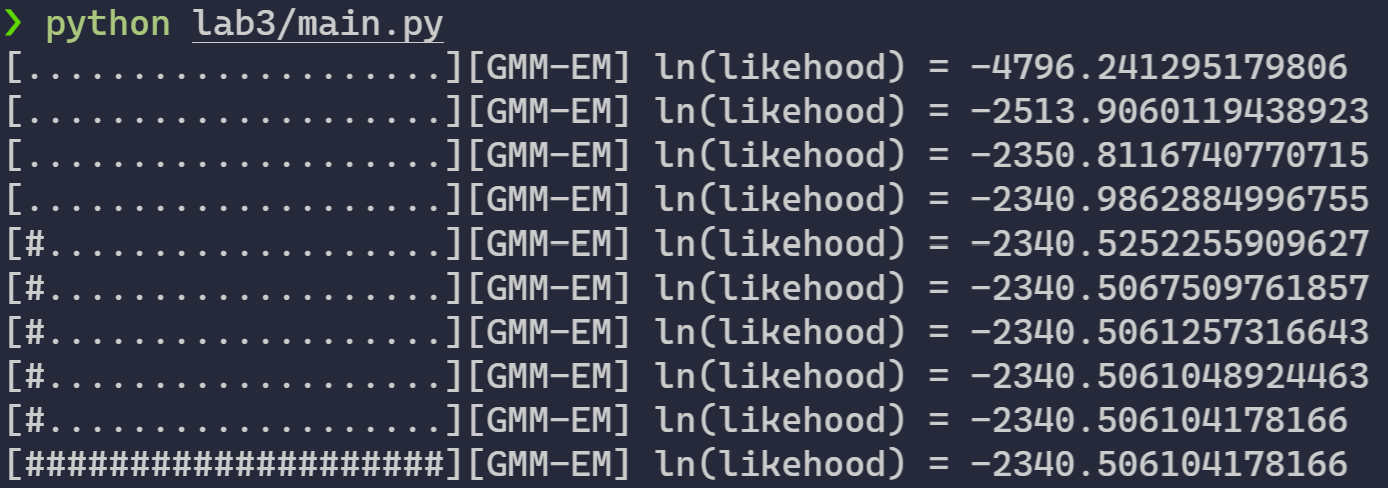
\includegraphics[width=\textwidth]{figures/Figure_15.png}
        \caption{$4$簇数据训练,各次迭代的对数似然 1}
    \end{minipage}
    \begin{minipage}[t]{0.5\linewidth}
        \centering
        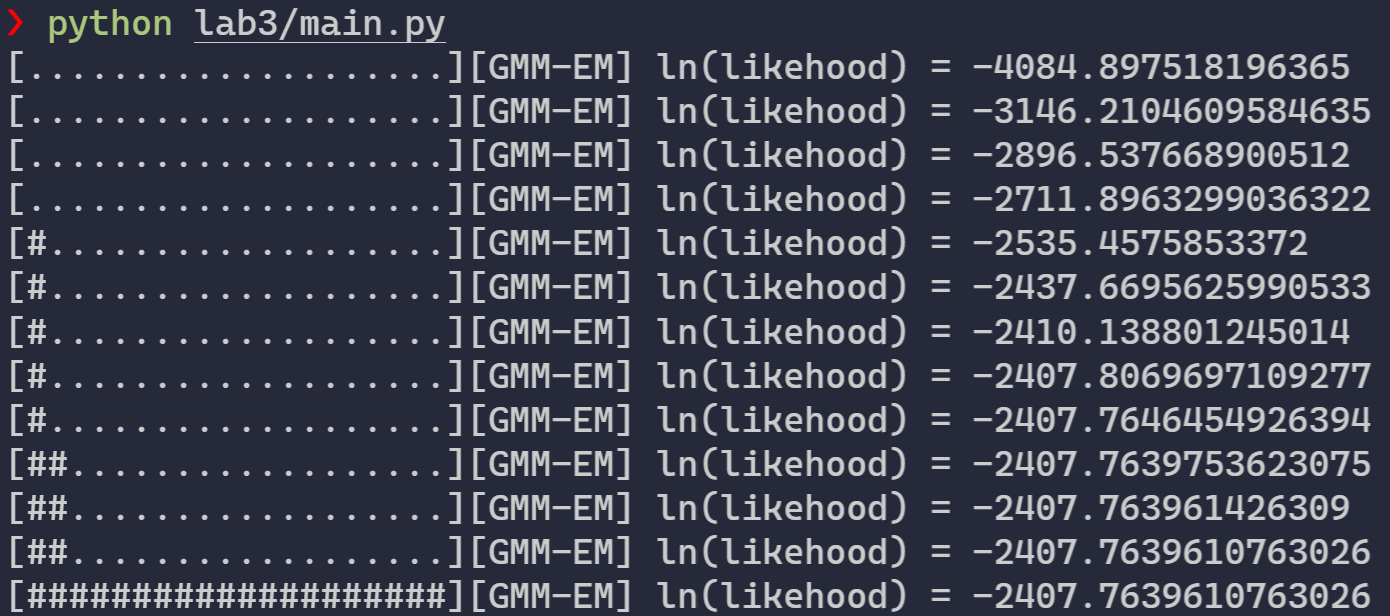
\includegraphics[width=\textwidth]{figures/Figure_16.png}
        \caption{$4$簇数据训练,各次迭代的对数似然 2}
    \end{minipage}
\end{figure}
\begin{figure}[htbp]
    \begin{minipage}[t]{0.5\linewidth}
        \centering
        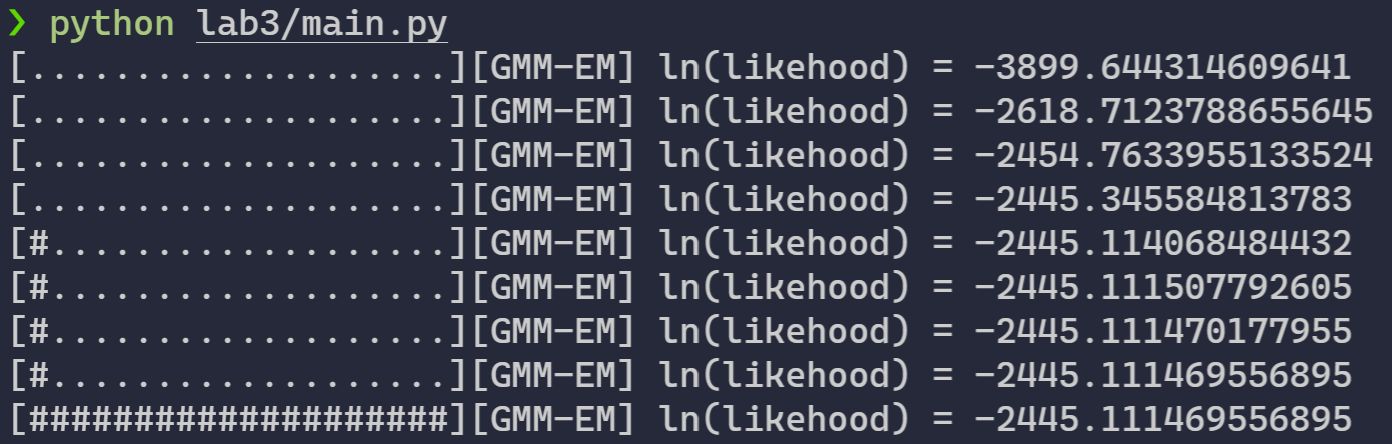
\includegraphics[width=\textwidth]{figures/Figure_17.png}
        \caption{$4$簇数据训练,各次迭代的对数似然 3}
    \end{minipage}
    \begin{minipage}[t]{0.5\linewidth}
        \centering
        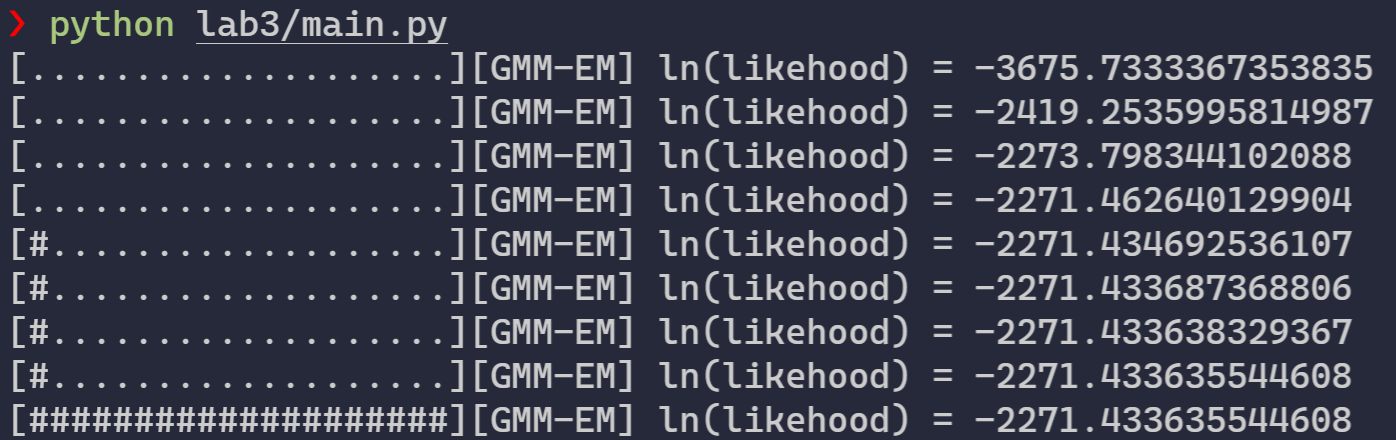
\includegraphics[width=\textwidth]{figures/Figure_18.png}
        \caption{$4$簇数据训练,各次迭代的对数似然 4}
    \end{minipage}
\end{figure}

可见GMM-EM在400组2维数据分4簇时,基本都能在10次迭代以内收敛,性能较好。

\subsection{UCI数据集测试}

使用UCI的iris数据集\cite{uci-iris},样本数据是4维的,不便于绘图。且由于样本数量较多、维度较高(4维),故在训练末期每次迭代后对数似然减小量较小,经常触发迭代次数上限。

选取的一次训练过程中的对数似然变化情况见附录,此次训练结果如图\ref{uci-iris}。

\begin{figure}[htbp]
    \centering
    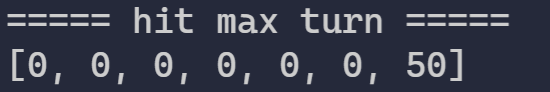
\includegraphics[width=0.7\textwidth]{figures/Figure_19.png}
    \caption{Iris数据集训练结果}
    \label{uci-iris}
\end{figure}

图\ref{uci-iris}表示用于测试的50个样本点全部被分到对应的簇6中,准确率为$100\%$。
